\chapter*{Trigonometría}
\setcounter{chapter}{1}
\setcounter{section}{0}

\section{Relaciones trigonométricas}
\begin{center}
    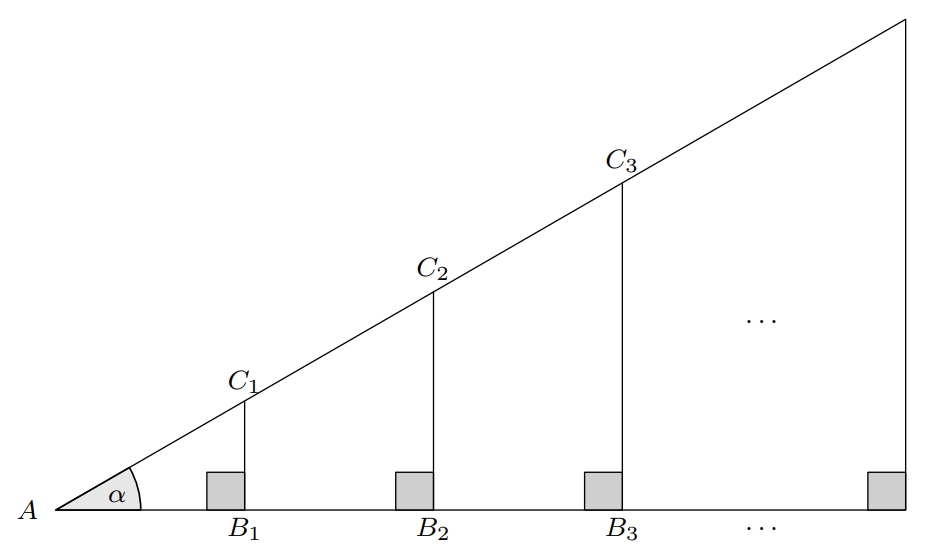
\includegraphics[width=0.8\linewidth]{trigonometria1.jpg}
\end{center}
Todos los tríangulos tienen el mismo ángulo agudo $\alpha$°.\\
Como todos los tríangulos respectivamente tienen igual medida, son \textbf{triángulos semejantes entre sí}. Es por esto que las razones entre los lados homólogos son iguales y solo dependen de la medida del $\angle A$
$$\frac{\overline{B_1 C_1}}{\overline{AB_1}} = \frac{\overline{B_2C_2}}{\overline{AB_2}} = \frac{\overline{B_3C_3}}{\overline{AB_3}} = \dots = k$$

\begin{center}
    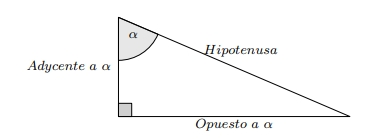
\includegraphics[width=0.6\linewidth]{trigonometria2.jpg}
\end{center}

\blueBox{Definición}{
    Dado un triángulo rectángulo donde uno de sus ángulos agudos es $\alpha$, se definen las siguientes relaciones:
    \begin{center}
        \begin{itemize}
            \item $\sin (\alpha) = \frac{\text{cat. opuesto a } \alpha}{\text{hipotenusa}}$
            \item $\cos(\alpha) = \frac{\text{cat. adyacente a } \alpha}{\text{hipotenusa}}$
            \item $\tan(\alpha) = \frac{\text{cat. opuesto a } \alpha}{\text{cat. adyacente a } \alpha}$ 
            \item $\text{cotg}(\alpha) = \frac{\text{cat. adyacente a } \alpha}{\text{cat. opuesto a } \alpha}$
            \item $\text{sec}(\alpha) = \frac{\text{hipotenusa}}{{\text{cat. adyacente a } \alpha}}$
            \item $\text{cosec}(\alpha) = \frac{\text{hipotenusa}}{\text{cat. opuesto a } \alpha}$ 
        \end{itemize}
    \end{center}
}

\textbf{Observación} \emph{De la definición se tiene que:}
$$cosec(\alpha) = \frac{\text{hipotenusa}}{\text{cat. opuesto a } \alpha} = \frac{1}{\frac{{\text{cat. opuesto a } \alpha}}{\text{hipotenusa}}} = \frac{1}{\sin (\alpha)}$$
También está:
$$sec(\alpha) = \frac{1}{cos(\alpha)} \;\;\;\;\; y \;\;\;\;\; cotg(\alpha) = \frac{1}{\tan(\alpha)}$$

\section{Valores de las razones trigonométricas de algunos ángulos}

\begin{enumerate}
    \item $\sin(30^\circ) = \frac{1}{2}$
    \item $\cos(30^\circ) = \frac{\sqrt{3}}{2}$
    \item $\tan(30^\circ) = \frac{\sin(30^\circ)}{\cos(30^\circ)} = \frac{\frac{1}{2}}{\frac{\sqrt{3}}{2}} = \frac{1}{\sqrt{3}}$
    \item $cosec(30^\circ) = \frac{1}{sen(30^\circ)} = 2$
    \item $sec(30^\circ) = \frac{1}{cos(30^\circ)} = \frac{2}{\sqrt{3}}$
    \item $cotg(30^\circ) = \frac{1}{tg(30^\circ)} = \sqrt{3}$
\end{enumerate}
Lo mismo para $60^\circ$
\begin{enumerate}
    \item $\sin(60^\circ) = \frac{\sqrt{3}}{2}$
    \item $\cos(60^\circ) = \frac{1}{2}$
    \item $\tan(60^\circ) = \frac{\sin(60^\circ)}{\cos(60^\circ)} = \frac{\frac{\sqrt{3}}{2}}{\frac{1}{2}} = \sqrt{3}$
    \item $cosec(60^\circ) = \frac{1}{sen(60^\circ)} = \frac{2}{\sqrt{3}}$
    \item $sec(60^\circ) = \frac{1}{cos(60^\circ)} = 2$
    \item $cotg(60^\circ) = \frac{1}{tg(60^\circ)} = \frac{1}{\sqrt{3}}$
\end{enumerate}
Y para $45^\circ$
\begin{enumerate}
    \item $\sin(45^\circ) = \frac{\sqrt{2}}{2}$
    \item $\cos(45^\circ) = \frac{\sqrt{2}}{2}$
    \item $\tan(45^\circ) = \frac{\sin(45^\circ)}{\cos(45^\circ)} = \frac{\frac{1}{\sqrt{2}}}{\frac{1}{\sqrt{2}}} = 1$
    \item $cosec(45^\circ) = \frac{1}{sen(45^\circ)} = \sqrt{2}$
    \item $sec(45^\circ) = \frac{1}{cos(45^\circ)} = \sqrt{2}$
    \item $cotg(45^\circ) = \frac{1}{tg(45^\circ)} = 1$
\end{enumerate}

\section{Cálculo de los ángulos conociendo los lados de un triángulo rectángulo}
Conociendo los lados de un triángulo rectángulo, se pueden calcular todos sus ángulos.

Por ejemplo:
\begin{center}
    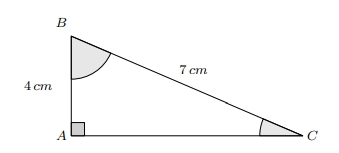
\includegraphics[width=0.6\linewidth]{trigonometria3.jpg}
\end{center}
Para calcular la medida de $\angle B$ se tiene que:
$$\cos(\angle B) = \frac{4}{7}$$
En la calculadora:
$$\boxed{SHIFT} + \boxed{cos} + \boxed{(4/7)}$$
da como resultado:
$$\angle B \approx 55,15^\circ$$
Y como $\angle B + \angle C = 90^\circ$ se tiene que:
$$\angle C = 90^\circ - 55,15^\circ = 34,85^\circ$$

\section{Relación pitagórica}
Esta relación nos permite relacionar el seno con el coseno de un mismo ángulo

\blueBox{Relación Pitagírica}{
    En todo triángulo rectángulo y para cualquiera de sus ángulos se verifica que:
    $$\sin^2(\alpha) + \cos^2(\alpha) = 1$$
    Aplicando las definiciones de seno y coseno:
    $$
    \begin{aligned}
        \sin^2(\alpha) + \cos^2(\alpha) &= \frac{(\text{cat. opuesto a } \alpha)^2}{\text{hipotenusa}^2} + \frac{(\text{cat. adyacente a } \alpha)^2}{\text{hipotenusa}^2} \\
        &= \frac{(\text{cat. opuesto a } \alpha)^2 + (\text{cat. adyacente a } \alpha)^2}{\text{hipotenusa}^2} \\
        &= \frac{(\text{hipotenusa})^2}{\text{hipotenusa}^2} \\
        &= 1
    \end{aligned}
    $$
}

\section{Circunferencia trigonométrica}
Teniendo una circunferencia de radio 1, con centro en el origen de coordenadas, el punto $P$ de coordenadas $(x, y)$ sobre la circunferencia y en el primer cuadrante y el segmento $OP$ que une el origen con $P$, se tiene que:
\begin{center}
    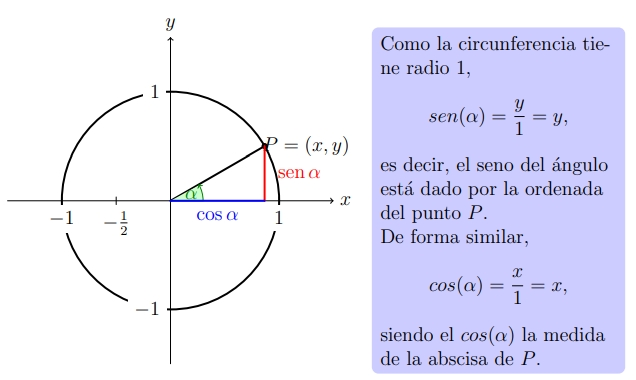
\includegraphics[width=0.8\linewidth]{trigonometria4.jpg}
\end{center}

\subsection{Ángulos importantes}
\begin{tabular}{c||c||c||c||c}
    {\bf Ángulo} & {\bf $0^\circ$} & {\bf $90^\circ$} & {\bf $180^\circ$} & {\bf $270^\circ$} \\
    \hline
    \hline
    {\bf $seno (y)$} & 0 & 1 & 0 & -1\\
    {\bf $coseno (x)$} & 1 & 0 & -1 & 0
\end{tabular}

\section{Algunas identidades importantes}
$$sen^2(\alpha) + cos^2(\alpha) = 1$$
$$tan(\alpha) = \frac{sen(\alpha)}{cos(\alpha)}$$
$$sen(90^\circ - \alpha) = cos(\alpha)$$

\subsection{Paridad e imparidad del seno y coseno}
Los ángulos "positivos" son cuando los medimos en sentido antihorario, y los "negativos" cuando los medimos en sentido horario.
$$cos(-\alpha) = cos(\alpha)$$
$$sen(-\alpha) = -sen(\alpha)$$

\subsection{Fórmulas de suma y resta}
$$sen(\alpha + \beta) = sen(\alpha) \cdot cos(\beta) + cos(\alpha) \cdot sen(\beta)$$
$$cos(\alpha + \beta) = cos(\alpha) \cdot cos(\beta) - sen(\alpha) \cdot sen(\beta)$$
$$sen(\alpha - \beta) = sen(\alpha) \cdot cos(\beta) - cos(\alpha) \cdot sen(\beta)$$
$$cos(\alpha - \beta) = cos(\alpha) \cdot cos(\beta) + sen(\alpha) \cdot sen(\beta)$$

\subsection{Ángulos suplementarios}
$$sen(180^\circ - \alpha) = sen(\alpha)$$
$$cos(180^\circ - \alpha) = -cos(\alpha)$$

\section{Área de un triángulo}
Sabiendo la medida de 2 de sus lados y un ángulo, se puede calcular el Área
\begin{center}
    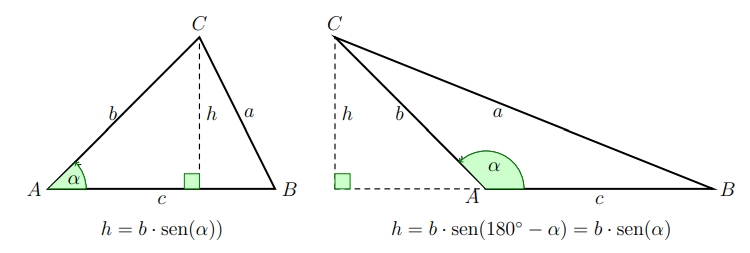
\includegraphics[width=0.8\linewidth]{trigonometria5.jpg}
\end{center}
Tanto si el triángulo es acutángulo como obtusángulo, tomando como "base" el lado $\overline{AB}$, la altura $h$ es:
$$h = b \cdot sen(\alpha)$$
Como el área de un triángulo es $\frac{Base \cdot h}{2}$, el área del triángulo $\triangle ABC$ es:
$$\left[\triangle ABC\right] = \frac{1}{2} b c sen(\alpha)$$
donde $\alpha$ es el ángulo entre $\overline{AB}$ y $\overline{AC}$

\section{Teoremas del seno y del coseno}
Estos teoremas nos permiten relacional las medidas de los lados y ángulos de un triángulo cualquiera. Generalizan la trigonometría a triángulos que no son necesariamente rectángulos
\blueBox{Teorema del Seno}{
    En todo tríangulo $\triangle ABC$ se verifica que 
    $$\frac{a}{sen(\alpha)} = \frac{b}{sen(\beta)} = \frac{c}{sen(\gamma)}$$
    Si además consideramos la circunferencia que inscribe al $\triangle ABC$, se verifica que
    $$\frac{a}{sen(\alpha)} = \frac{b}{sen(\beta)} = \frac{c}{sen(\gamma)} = 2r$$
}

\blueBox{Teorema del Coseno}{
    En todo triángulo $\triangle ABC$ se verifica que
    $$a^2 = b^2 + c^2 - 2bc \cdot cos(\angle A)$$
}

\section{Pendiente de una recta}
Sea $f(x) = ax+b$ una función lineal. La pendiente nos indica la variación de la función cuando la variable independiente aumenta en 1 unidad. La pendiente de la recta es:
$$f(x+1) - f(x) = a \;\;\;\;\;\;\; \forall x \in \R$$
\begin{center}
    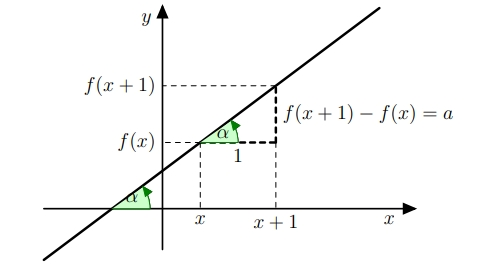
\includegraphics[width=0.8\linewidth]{trigonometria6.jpg}
\end{center}
Por la definición de tangente se tiene que la pendiente de una recta es la tangente del ángulo que forma con el semieje positivo de las abscisas:
$$\boxed{a = tan(\alpha)}$$
